\section{The temperature dependence of the many-particle entanglement}
\label{sec:entanglement}
We use  the second moment $M_2$ of Eq. ~(\ref{eq:dispersion}) for the investigation of the many-particle entanglement in a spin system of 201 spins. 
The intensities of the reduced MQ NMR coherences are determined by Eqs.  ~(\ref{eq:j_lt},~\ref{eq:j_lt_norm}) both at high ($b < 1$) and low ($b > 1$) temperatures. 
We start from $b = 0.1$, which corresponds to the temperature ${T= 2.4\cdot 10^{-1}}$~K at the Larmor frequency $\omega_0 = 2\pi\cdot 500\cdot10^6$ s$^{-1}$ (Fig.~\ref{fig:m2_t_b01}). 
The inequality~(\ref{eq:fisher_criteria}) can be satisfied only when $k=1$ (the horizontal line on Fig.~\ref{fig:m2_t_b01}). 
This means pair entanglement is possible in the high-temperature case \cite{lab:mq_mnr_qinfo_2012}. \begin{figure}
    \centering
    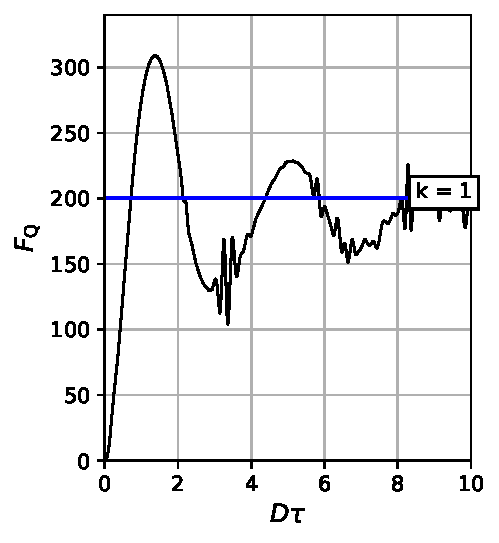
\includegraphics{pic/m2_t_b01.pdf}
    \caption{The dependence of the lower bound for the quantum Fisher information $F_Q = 2M_2(\tau)$ on the dimensionless time $D\tau$ at ${T=2.4\cdot10^{-1}}$~K $(b=0.1)$. 
    The inequality~(\ref{eq:fisher_criteria}) yields the region of pair entanglement $(k+1=2)$. The region is above the horizontal line. 
    }
    \label{fig:m2_t_b01}
\end{figure}
\par 
At the temperature ${4.8\cdot10^{-2}}$~K $(b=0.5)$ one can see a strip (Fig.~\ref{fig:m2_t_b05}), in which the inequality~(\ref{eq:fisher_criteria}) can be satisfied when $14 \leq k \leq 27$.
\begin{figure}
    \centering
    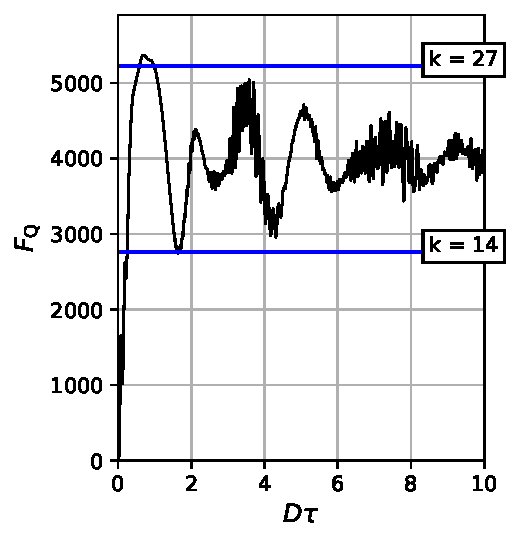
\includegraphics{pic/m2_t_b05.pdf}
    \caption{The dependence of the lower bound for the quantum Fisher information on the dimensionless time $D\tau$ at ${T=4.8\cdot10^{-2}}$~K $(b=0.5)$. The region of the many-spin entanglement is a strip bounded by the horizontal lines with $k=14$ and $k=27$.}
    \label{fig:m2_t_b05}
\end{figure}
Thus, there is many-spin entanglement in spin clusters consisting of 15 to 28 spins at the temperature  ${4.8\cdot10^{-2}}$~K. When the temperature decreases, the width of the strip, where many-spin entanglement exists, increases. At the temperature ${2.4\cdot10^{-2}}$~K $(b=1)$ (Fig.~\ref{fig:m2_t_b1}), in such a strip, the number of the entangled spins can range from 36 to 92.
\begin{figure}
    \centering
    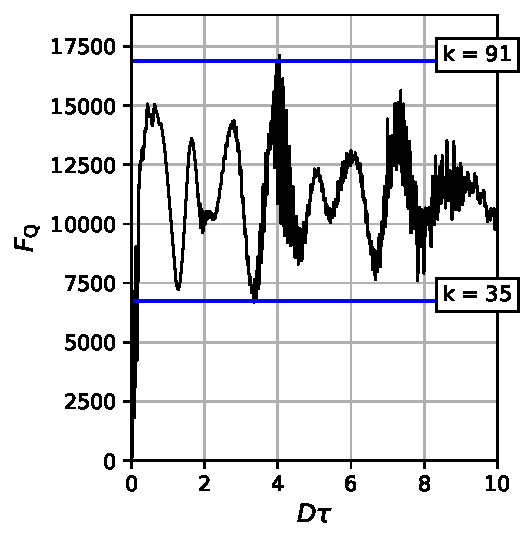
\includegraphics{pic/m2_t_b1.pdf}
    \caption{The dependence of the lower bound for the quantum Fisher information on the dimensionless time $D\tau$ at ${T=2.4\cdot10^{-2}}$~K $(b=1)$. The horizontal lines bound the strip with the many-spin entanglement.}
    \label{fig:m2_t_b1}
\end{figure}
\par
Finally, at the temperature ${T= 6.856\cdot10^{-3}}$~K $(b=3.5)$ (Fig.~\ref{fig:m2_t_b3.5}), almost all spins (up to 179 of 201) are entangled. Entanglement exists during  the evolution process except a short initial period of time. 
\begin{figure}
    \centering
    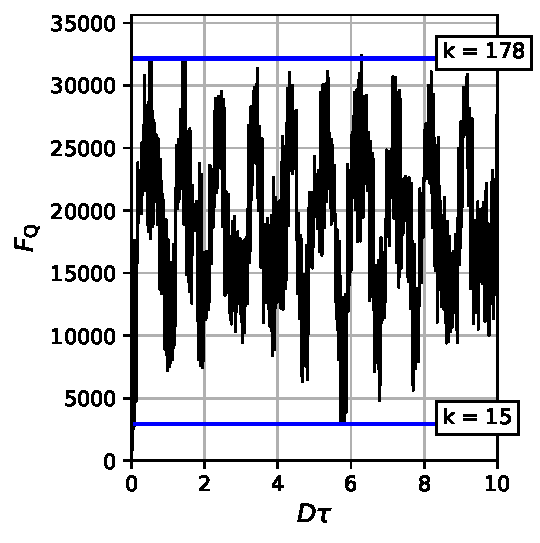
\includegraphics{pic/m2_t_b3_5.pdf}
    \caption{The dependence of the lower bound for the quantum Fisher information on the dimensionless time $D\tau$ at ${T=6.856\cdot10^{-3}}$~K $(b=3.5)$.
    Almost all spins (up to $179$ of $201$) can be a part of the entangled cluster.}
    \label{fig:m2_t_b3.5}
\end{figure}
\par 
Fig.\ref{fig:k_b} demonstrates that the number of the entangled spins increases when the temperature decreases.
\par
Thus, the suggested model of a nanocavity filled with spin-carrying atoms (molecules) allows us to investigate many-spin entanglement and its dependence on the temperature.
\begin{figure}
    \centering
    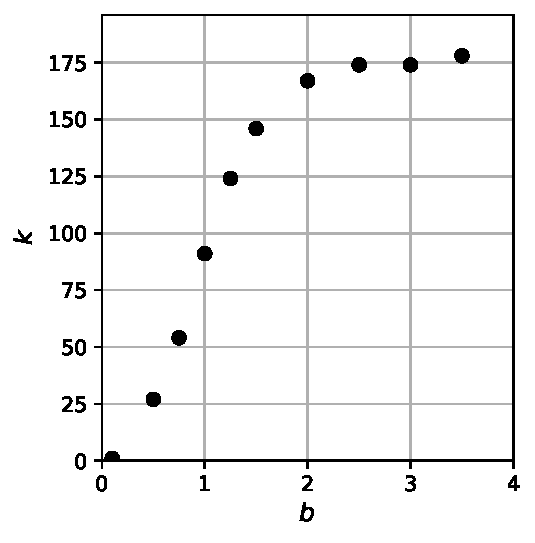
\includegraphics{pic/k_b.pdf}
    \caption{The dependence of the number of the entangled spins on the parameter $b = \frac{\hbar\omega_0}{kT} $.}
    \label{fig:k_b}
\end{figure}
